
% This LaTeX was auto-generated from MATLAB code.
% To make changes, update the MATLAB code and republish this document.

\documentclass{article}
\usepackage{graphicx}
\usepackage{color}

\sloppy
\definecolor{lightgray}{gray}{0.5}
\setlength{\parindent}{0pt}

\begin{document}

    
    
\subsection*{Contents}

\begin{itemize}
\setlength{\itemsep}{-1ex}
   \item Problem 1
   \item GENERATE TRAJECTORY Problem 2
   \item Implement the inverse dynamic control  Problem 3
   \item Plotting the result: please plot both the actual trajectory and the desired trajectory for the your states. example code below.
   \item With different initial condition
   \item Bonus problem
   \item With different initial condition
\end{itemize}
\begin{verbatim}
%%Farid Tavakkolmoghaddam
clc
clear all;
close all;
% the following parameters for the arm
I1=10;  I2 = 10; m1=5; r1=.5; m2=5; r2=.5; l1=1; l2=1;
g=9.8;

% we compute the parameters in the dynamic model
a = I1+I2+m1*r1^2+ m2*(l1^2+ r2^2);
b = m2*l1*r2;
d = I2+ m2*r2^2;
\end{verbatim}


\subsection*{Problem 1}

\begin{verbatim}
%initial state
tt0=0;
qq0=[pi*180/pi pi/2*180/pi 0 0];
% final state
ttf=5; % time span is 10 seconds
qqf=[0 0 0 0];
options = odeset('RelTol',1e-4,'AbsTol',[1e-4, 1e-4, 1e-4, 1e-4]);
[T0,X0] = ode45(@(t,x) feedback(t,x),[tt0 ttf],qq0, options);
figure('Name','Theta_1 using set point controller');
plot(T0, X0(:,1),'k');
title('Theta_1 using set point controller')
xlabel('Time (s)')
ylabel('Position (degree)')
grid on
hold on
figure('Name','Theta_2 using set point controller');
plot(T0, X0(:,2),'k');
title('Theta_2 using set point controller')
xlabel('Time (s)')
ylabel('Position (degree)')
grid on
hold on
\end{verbatim}

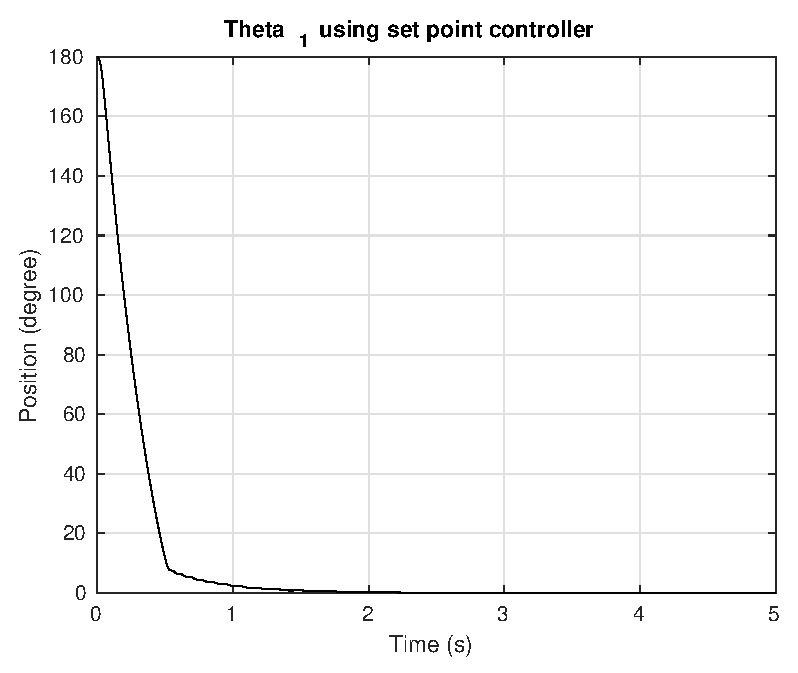
\includegraphics [width=4in]{TwoLinkArm_01.eps}

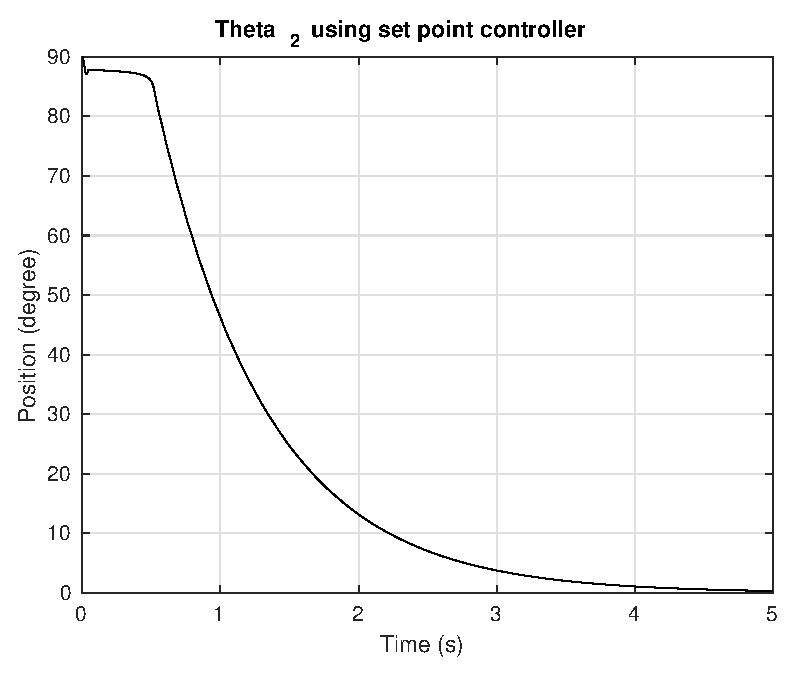
\includegraphics [width=4in]{TwoLinkArm_02.eps}


\subsection*{GENERATE TRAJECTORY Problem 2}

\begin{par}
initial state
\end{par} \vspace{1em}
\begin{verbatim}
t0=0;
q0=[0 0 0 0];
% final state
tf=10; % time span is 10 seconds
qf=[pi/3*180/pi pi/4*180/pi 0 0];
% generating the desired trajectory based on the initial and terminal
% state conditions
[link1,position1,velocity1,t]= TajectoryGenerator( q0(1), q0(3), qf(1), qf(3),t0,tf);
[link2,position2,velocity2,t]= TajectoryGenerator( q0(2), q0(4), qf(2), qf(4),t0,tf);
\end{verbatim}

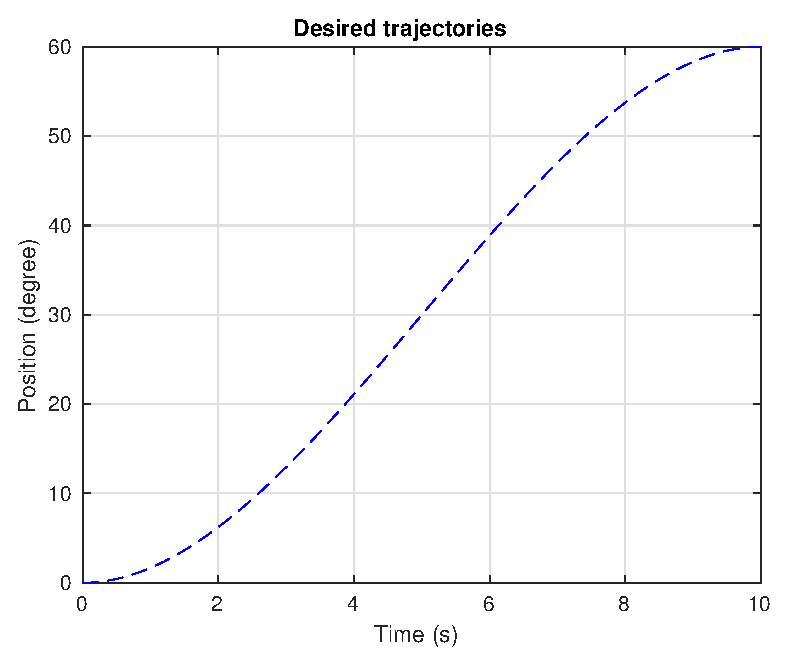
\includegraphics [width=4in]{TwoLinkArm_03.eps}

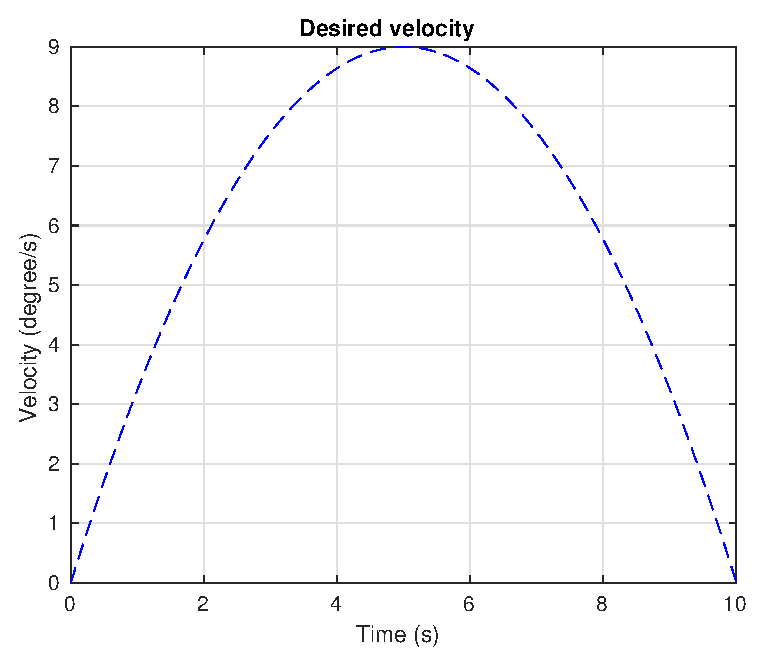
\includegraphics [width=4in]{TwoLinkArm_04.eps}

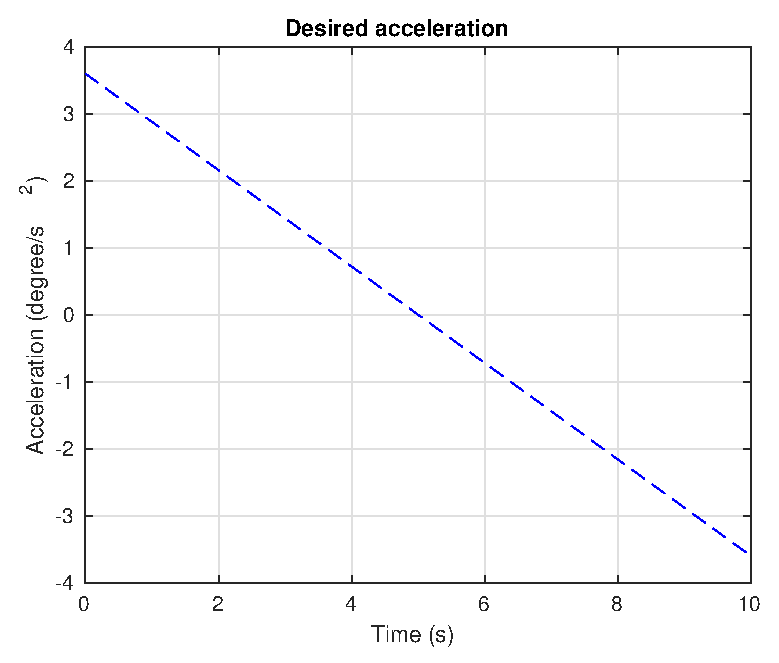
\includegraphics [width=4in]{TwoLinkArm_05.eps}

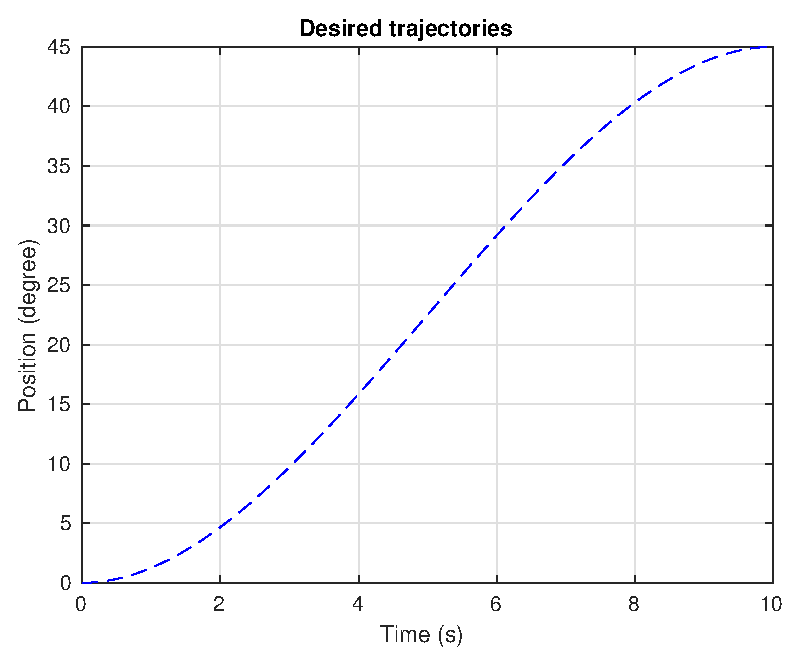
\includegraphics [width=4in]{TwoLinkArm_06.eps}

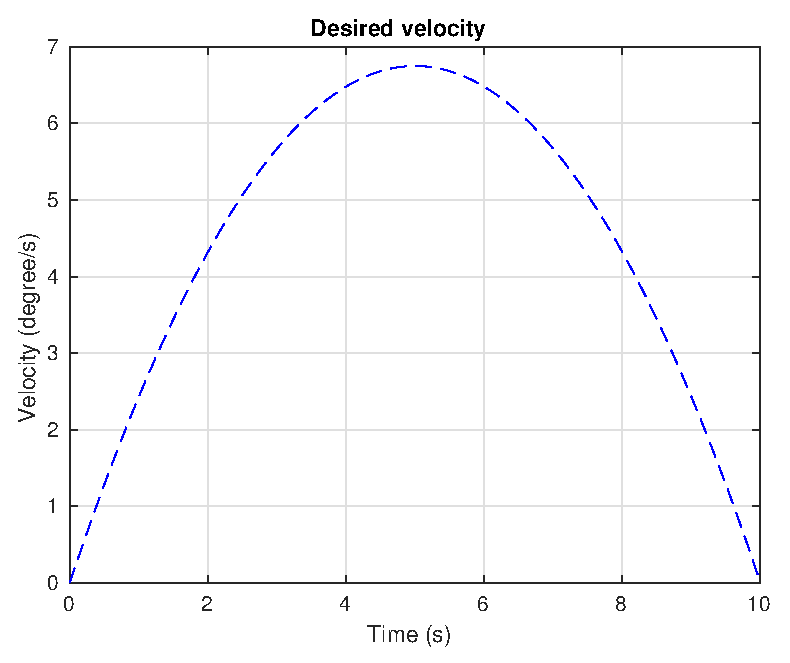
\includegraphics [width=4in]{TwoLinkArm_07.eps}

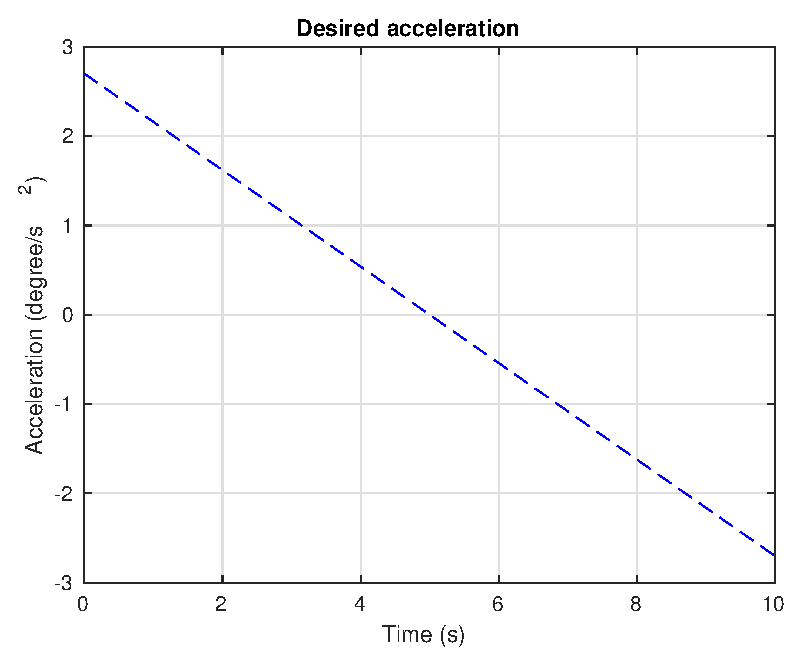
\includegraphics [width=4in]{TwoLinkArm_08.eps}


\subsection*{Implement the inverse dynamic control  Problem 3}

\begin{verbatim}
integral_term=false; % this is used for using the integration term for the controller
options = odeset('RelTol',1e-4,'AbsTol',[1e-4, 1e-4, 1e-4, 1e-4]);
[T,X] = ode45(@(t,x) inverseDC(t,x,link1,link2,integral_term),[0 tf],q0, options);
[T1,X1] = ode45(@(t,x) inverseDC(t,x,link1,link2,integral_term),[0 tf],[15 15 2 1.5], options);% starting with a different intial condition
\end{verbatim}


\subsection*{Plotting the result: please plot both the actual trajectory and the desired trajectory for the your states. example code below.}

\begin{verbatim}
figure('Name','Theta_1 under inverse dynamic control');
plot(T, X(:,1),'k--',t,position1,'b');
title('Theta_1 vs. Theta_1 desired using Trajectory tracking controller')
xlabel('Time (s)')
ylabel('Postion(degree)')
grid on
legend('actual','desired')
hold on
figure('Name','Theta_2 under inverse dynamic control');
plot(T, X(:,2),'k--',t,position2,'b');
title('Theta_2 vs. Theta_2 desired using Trajectory tracking controller')
xlabel('Time (s)')
ylabel('Postion(degree)')
grid on
legend('actual','desired')
hold on
% Plotting the Deired velocity Vs. Actual velocity
figure('Name','dTheta_1 vs. dTheta_1 desired under inverse dynamic control');
plot(T, X(:,3),'k--',t,velocity1,'b');
title('dTheta_1 vs. dTheta_1 desired using Trajectory tracking controller')
xlabel('Time (s)')
ylabel('Velocity(degree/s)')
legend('actual','desired')
grid on
hold on
figure('Name','Theta_2 under inverse dynamic control');
plot(T, X(:,4),'k--',t,velocity2,'b');
title('dTheta_2 vs. dTheta_2 desired using Trajectory tracking controller')
xlabel('Time (s)')
legend('actual','desired')
ylabel('Velocity(degree/s)')
grid on
hold on
\end{verbatim}

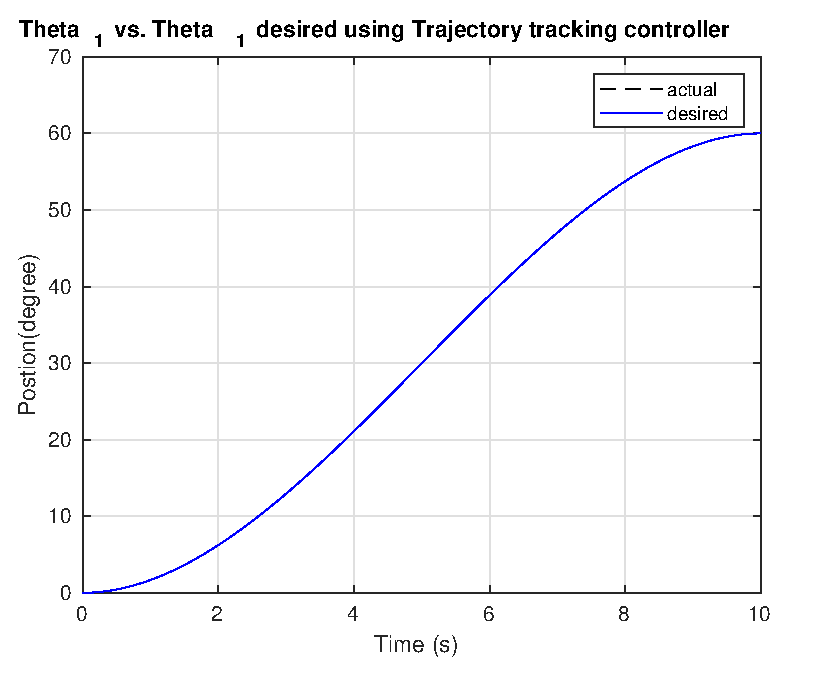
\includegraphics [width=4in]{TwoLinkArm_09.eps}

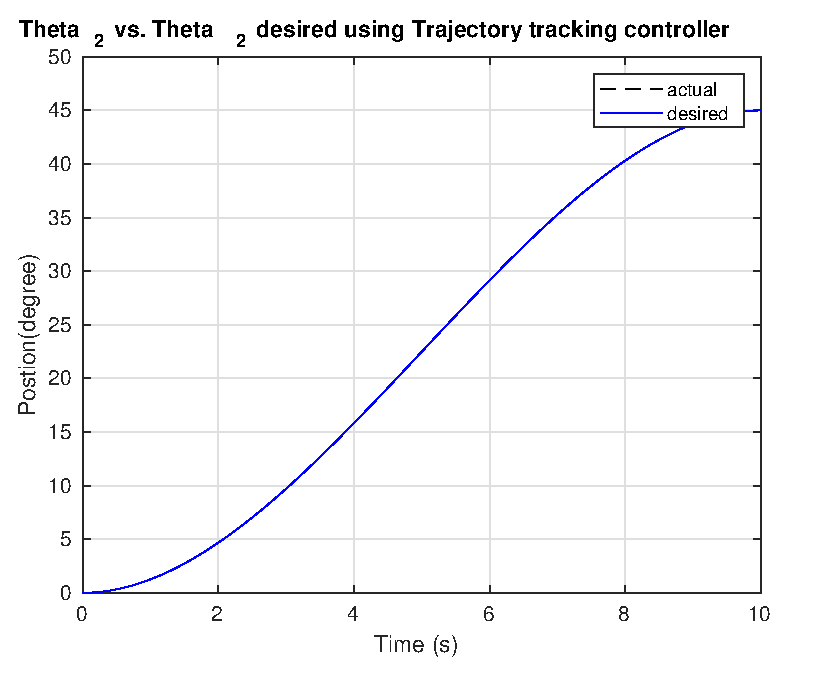
\includegraphics [width=4in]{TwoLinkArm_10.eps}

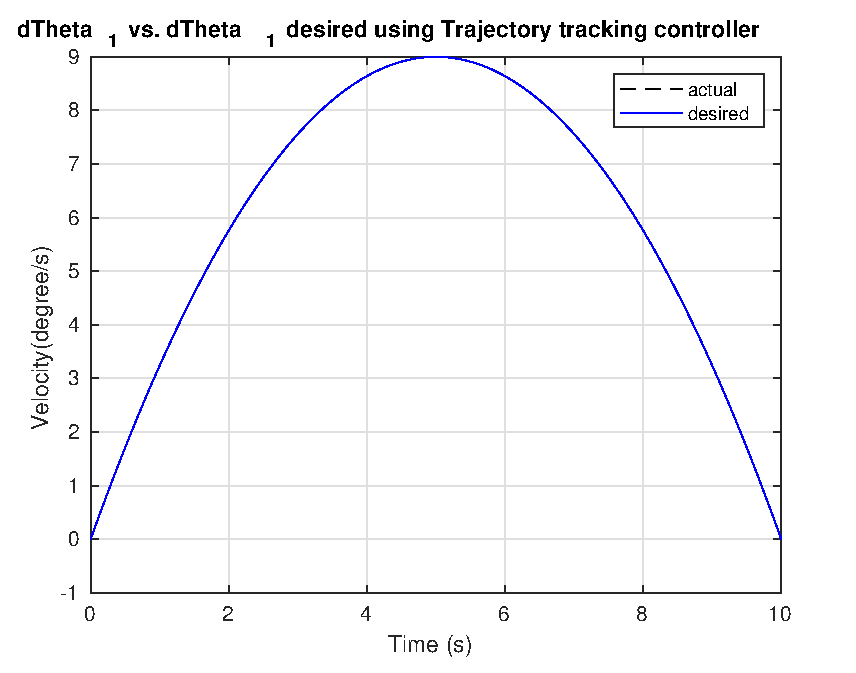
\includegraphics [width=4in]{TwoLinkArm_11.eps}

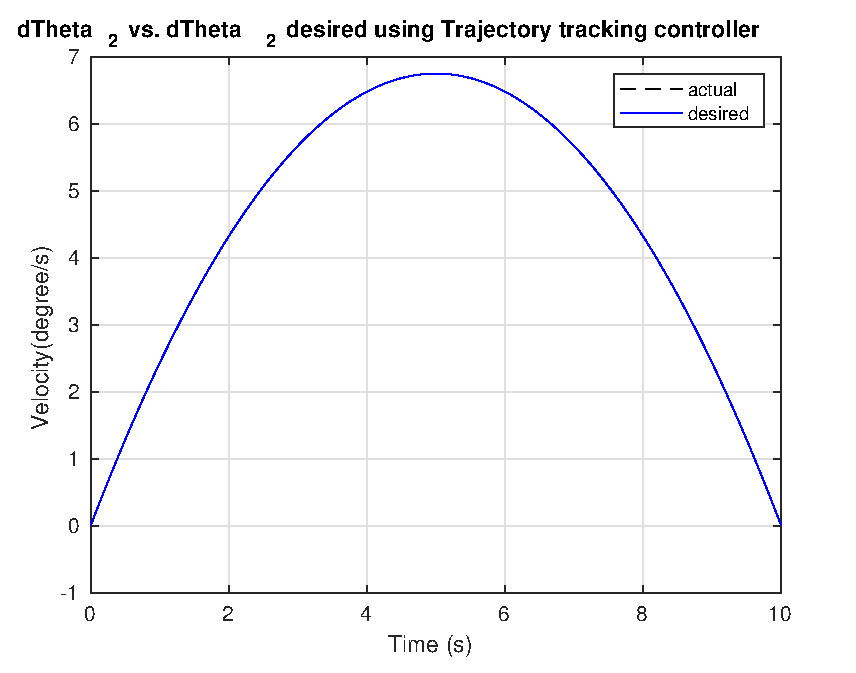
\includegraphics [width=4in]{TwoLinkArm_12.eps}


\subsection*{With different initial condition}

\begin{verbatim}
figure('Name','Theta_1 under inverse dynamic control');
plot(T1, X1(:,1),'r*',t,position1,'b');
title('Theta_1 vs. Theta_1 desired using Trajectory tracking controller')
xlabel('Time (s)')
ylabel('Position (degree)')
legend('actual','desired')
grid on
hold on
figure('Name','Theta_2 under inverse dynamic control');
plot(T1, X1(:,2),'r*',t,position2,'b');
title('Theta_2 vs. Theta_2 desired using Trajectory tracking controller')
xlabel('Time (s)')
ylabel('Position (degree)')
grid on
legend('actual','desired')
hold on
%
% Plotting the Deired velocity Vs. Actual velocity
figure('Name','Theta_1 under inverse dynamic control');
plot(T1, X1(:,3),'k--',t,velocity1,'b');
title('dTheta_1 vs. dTheta_1 desired using Trajectory tracking controller')
xlabel('Time (s)')
ylabel('Velocity(degree/s)')
legend('actual','desired')
grid on
hold on
figure('Name','Theta_2 under inverse dynamic control');
plot(T1, X1(:,4),'k--',t,velocity2,'b');
title('dTheta_2 vs. dTheta_2 desired using Trajectory tracking controller')
xlabel('Time (s)')
ylabel('Velocity(degree/s)')
legend('actual','desired')
grid on
hold on
\end{verbatim}

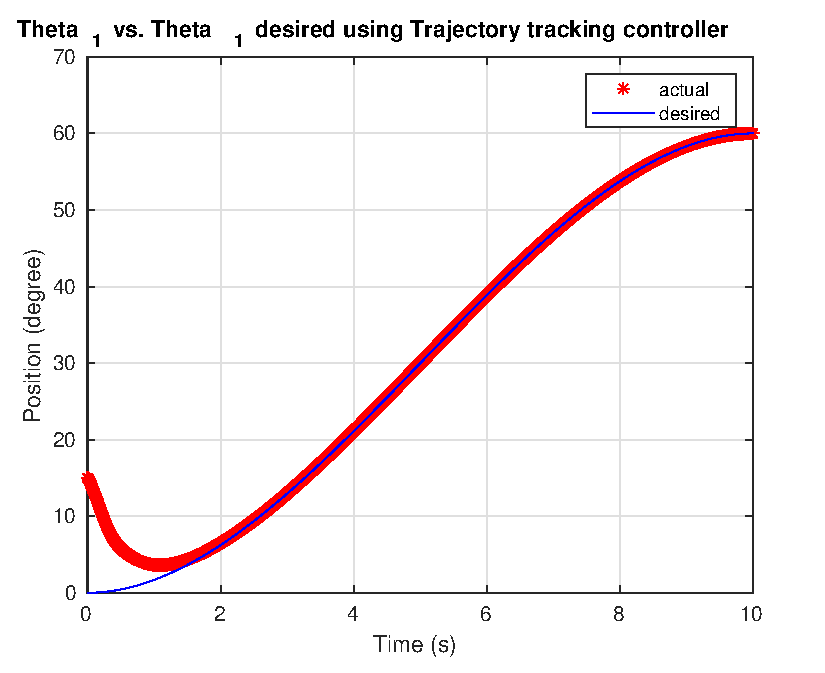
\includegraphics [width=4in]{TwoLinkArm_13.eps}

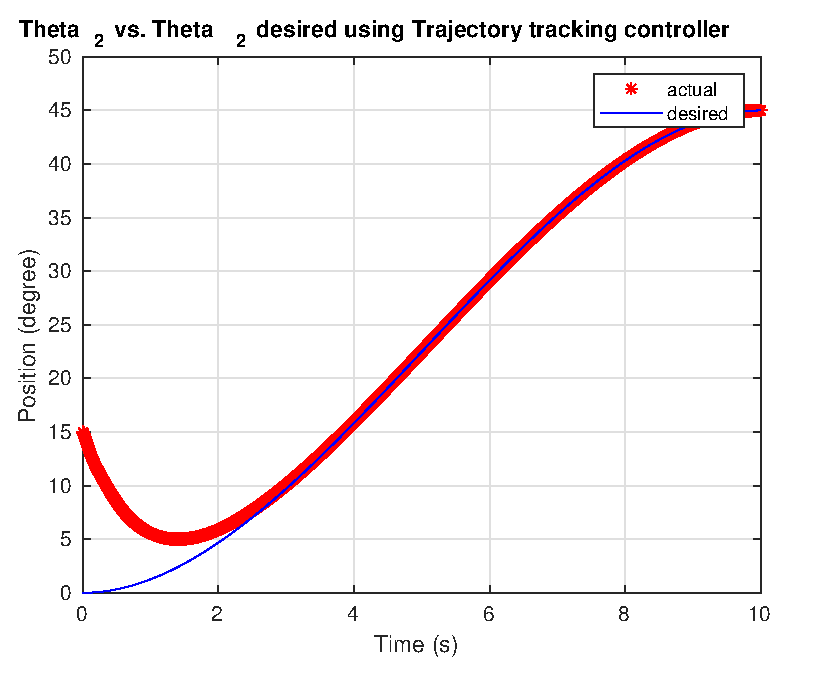
\includegraphics [width=4in]{TwoLinkArm_14.eps}

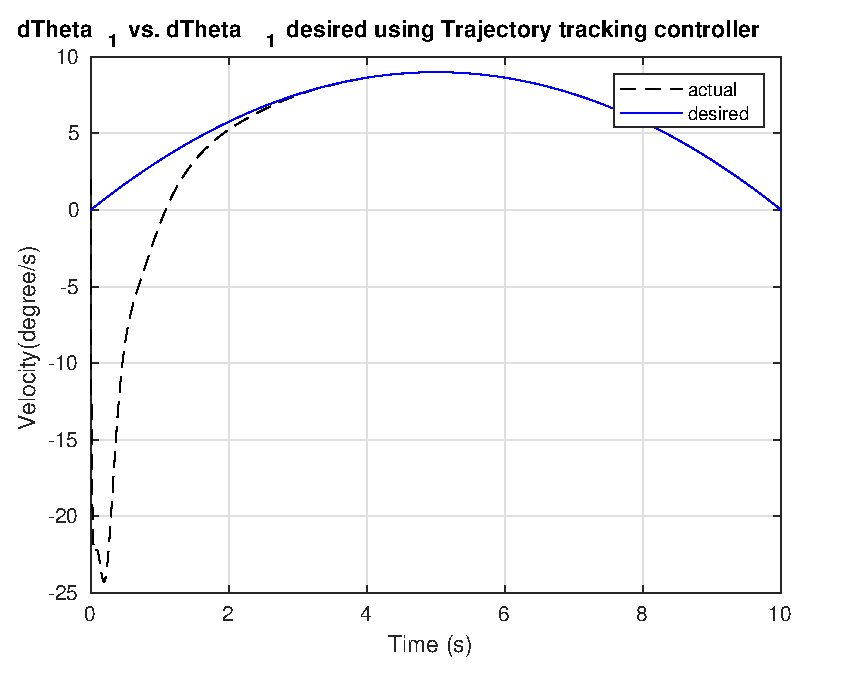
\includegraphics [width=4in]{TwoLinkArm_15.eps}

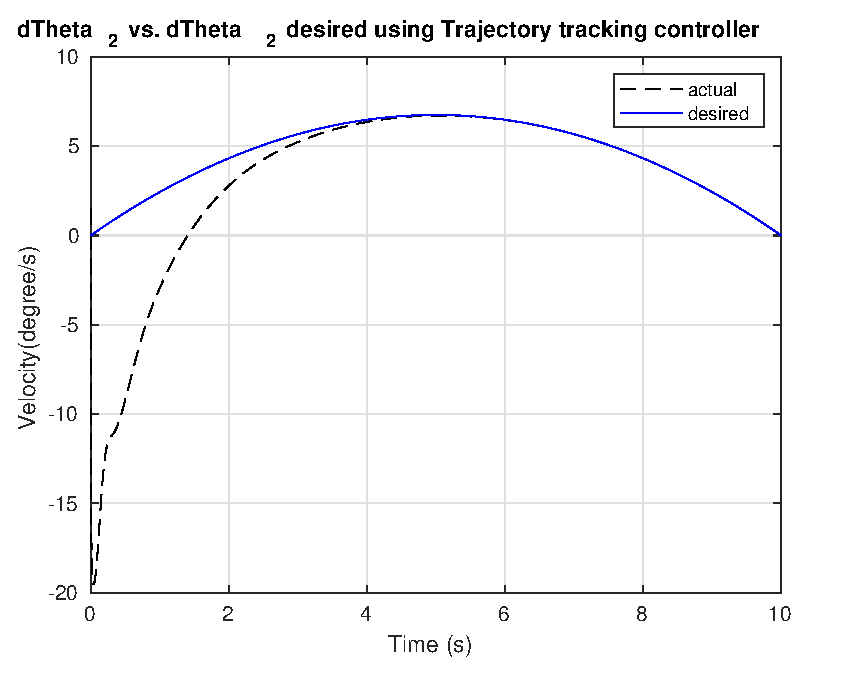
\includegraphics [width=4in]{TwoLinkArm_16.eps}


\subsection*{Bonus problem}

\begin{par}
setting the integration term to true so that we could enable the integrtion in the controller feedback.
\end{par} \vspace{1em}
\begin{verbatim}
integral_term=true;
options = odeset('RelTol',1e-4,'AbsTol',[1e-4, 1e-4, 1e-4, 1e-4]);
[T2,X2] = ode45(@(t,x) inverseDC(t,x,link1,link2,integral_term),[0 tf],q0, options);
figure('Name','Theta_1 under inverse dynamic control');
title('Theta_1 CTC controller with Ki term active')
plot(T2, X2(:,1),'k--',t,position1,'b');
legend('actual','desired')
grid on
hold on
figure('Name','Theta_2 under inverse dynamic control');
plot(T2, X2(:,2),'k--',t,position2,'b');
title('Theta_2 CTC controller with Ki term active')
legend('actual','desired')
grid on
hold on
\end{verbatim}

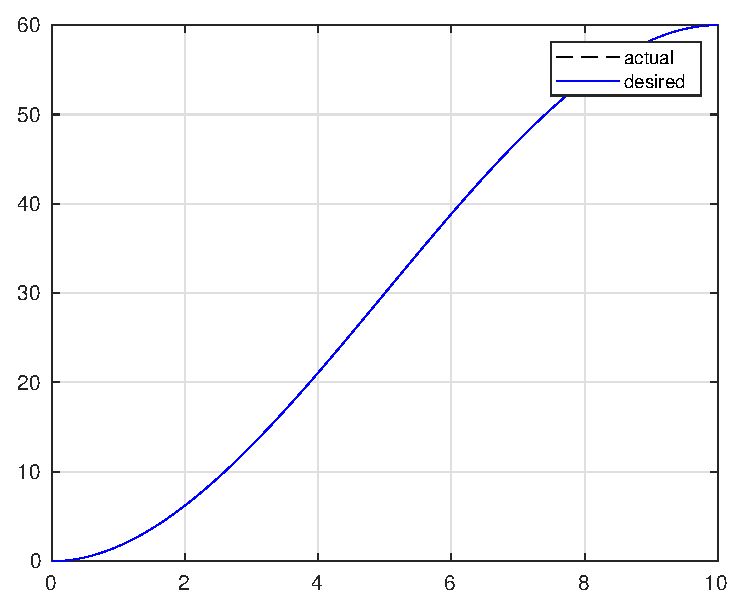
\includegraphics [width=4in]{TwoLinkArm_17.eps}

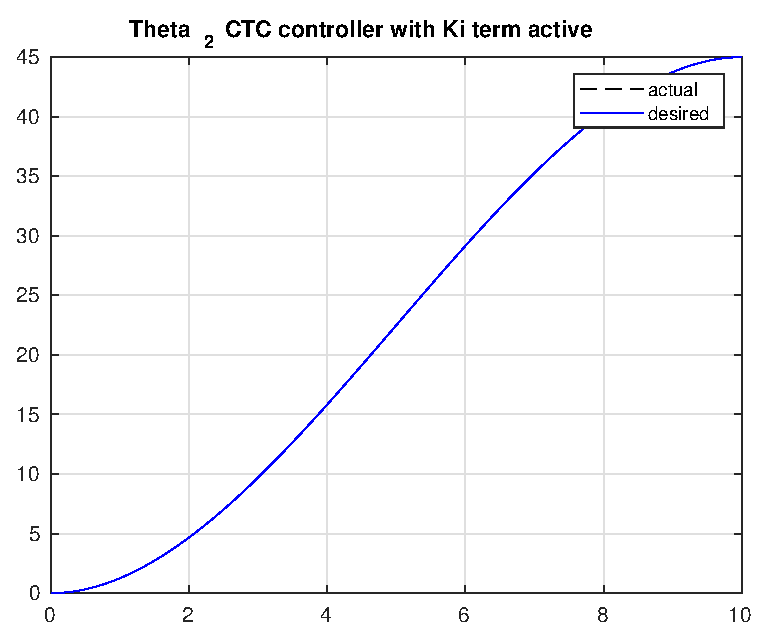
\includegraphics [width=4in]{TwoLinkArm_18.eps}


\subsection*{With different initial condition}

\begin{verbatim}
options = odeset('RelTol',1e-4,'AbsTol',[1e-4, 1e-4, 1e-4, 1e-4]);
[T3,X3] = ode45(@(t,x) inverseDC(t,x,link1,link2,integral_term),[0 tf],[20 15 1 5], options);
figure('Name','Theta_1 CTC controller with Ki term active');
plot(T3, X3(:,1),'r*',t,position1,'b');
title('Theta_1 CTC controller with Ki term active')
legend('actual','desired')
xlabel('Time (s)')
ylabel('Position (degree)')
grid on
hold on
figure('Name','Theta_2 CTC controller with Ki term active');
plot(T3, X3(:,2),'r*',t,position2,'b');
title('Theta_2 CTC controller with Ki term active')
legend('actual','desired')
xlabel('Time (s)')
ylabel('Position (degree)')
grid on
legend('actual','desired')
hold on
\end{verbatim}

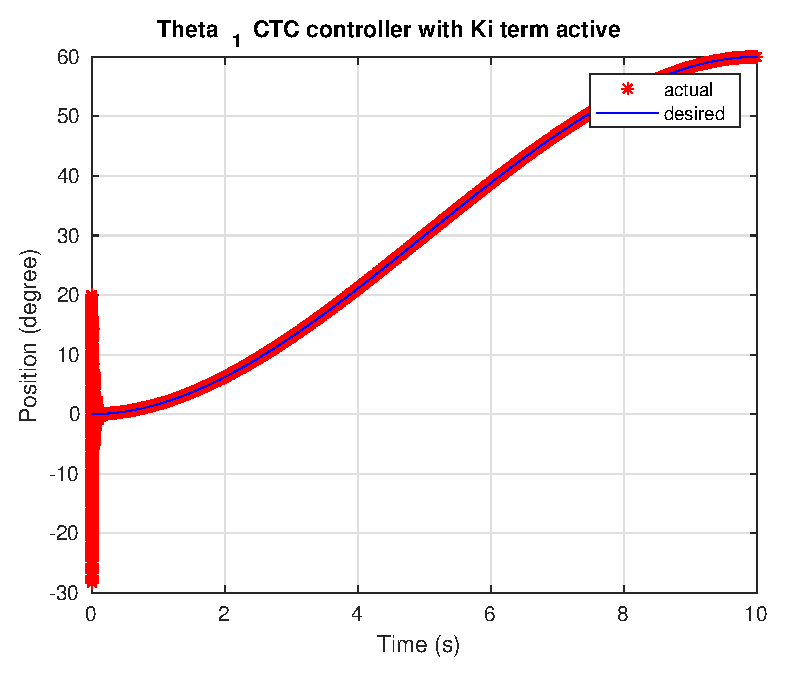
\includegraphics [width=4in]{TwoLinkArm_19.eps}

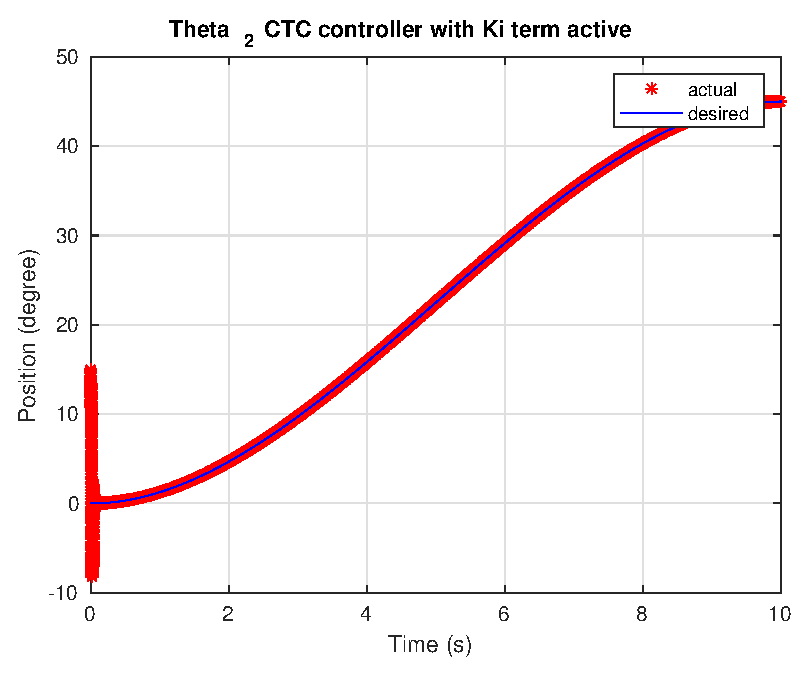
\includegraphics [width=4in]{TwoLinkArm_20.eps}



\end{document}
    
